% ========== Template by IC\M/T Institute of Creative\Media/Technologies =============
% ==========  M. Wagner and K. Blumenstein, N. Thuer 2017 ============= 
% ==========  Based on the LaTeX Thesis Template for the University of Applied Sciences St.Pölten by P. Lechner https://github.com/hrtlacek/ThesisTemplate-FH-StP        ============= 

%----------------------------------------------------------------
% TODO List


%----------------------------------------------------------------

%Dokumentklasse without end dot ;-)
\documentclass[a4paper,twoside,13pt, numbers=noenddot]{scrreprt}
\usepackage[left= 3.5cm,right = 3cm, bottom = 3.5 cm, top = 3 cm]{geometry}
\usepackage[onehalfspacing]{setspace}

% Standard Packages
\usepackage[utf8]{inputenc}

% ============= Settings for the Work =============

\def\workTitle{<Title of the Work>}
\def\subTitle{~}
\def\specialization{<Name of Masterclass>}
\def\studentFirstName{<FirstName>}
\def\studentLastName{<LastName>}
\def\studentId{<StudentID>}
\def\advisorPreTitle{<Pre-Title>}
\def\advisoFirstName{<FirstName>}
\def\advisorLastName{<LastName>}
\def\advisorPosTitle{<Pos-Title>}
\def\assessorPreTitle{<Pre-Title>}
\def\assessorFirstName{<FirstName>}
\def\assessorLastName{<LastName>}
\def\assessorPosTitle{<Pos-Title>}
\def\place{<Place>}
\def\dateDay{<DD>}
\def\dateMonth{<MM>}
\def\dateYear{<YYYY>}

\newif\ifuseGermanVersion				    % <== DONT TOUCH THIS!!!
\newif\ifuseMasterInteractiveTechnologies 	% <== CAN'T TOUCH THIS!!! (da da dada)
\newif\ifuseMasterDigitalDesign	            % <== DONT TOUCH THIS!!!
\newif\ifuseMasterDigitalMediaProduction	% <== DONT TOUCH THIS!!!
\newif\ifuseMasterDigitalHealthCare			% <== DONT TOUCH THIS!!!
\newif\ifuseBachelorMediaTechnologiesOne    % <== DONT TOUCH THIS!!!
\newif\ifuseBachelorMediaTechnologiesTwo    % <== DONT TOUCH THIS!!!
\newif\ifuseBachelorSmartEngineeringOne     % <== DONT TOUCH THIS!!!
\newif\ifuseBachelorSmartEngineeringTwo     % <== DONT TOUCH THIS!!!

%***************************************************************************************
% To switch the version please use the comment "%" option :-). After a language change, you have to rebuild the whole project (in Overleaf --> recompile from scratch) 
%\useGermanVersiontrue					    % German version
\useGermanVersionfalse					    % English version
%***************************************************************************************
% To switch between the study programs use the comment option :-) 
% !!!ATTENTION: Only one has to be activated!!!
\useBachelorMediaTechnologiesOnetrue		% Bachelor #1 Media Technology
%\useBachelorMediaTechnologiesTwotrue		% Bachelor #2 Media Technology
%\useMasterInteractiveTechnologiestrue		% Master Interactive Technologies
%\useMasterDigitalDesigntrue		        % Master Digital Design
%\useMasterDigitalMediaProductiontrue		% Master Digital Media Production
%\useMasterDigitalHealthCaretrue			% Master Digital Health Care
% \useBachelorSmartEngineeringOnetrue		% Bachelor #1 Smart Engineering
%\useBachelorSmartEngineeringTwotrue		% Bachelor #2 Smart Engineering
%***************************************************************************************

% ============= Packages =============

% Dokumentinformationen
\usepackage[
	pdftitle={\workTitle},
	pdfsubject={},
	pdfauthor={\studentFirstName \studentLastName},
	pdfkeywords={}
	pdftex=true, 
	colorlinks=true,
 	breaklinks=true,
	citecolor=black,
	linkcolor=black,	
	menucolor=black,	
	urlcolor=black
]{hyperref}

\hypersetup{
    bookmarks=true,         % show bookmarks bar?
    unicode=false,          % non-Latin characters in Acrobat’s bookmarks
    pdftoolbar=true,        % show Acrobat’s toolbar?
    pdfmenubar=true,        % show Acrobat’s menu?
    pdffitwindow=false,     % window fit to page when opened
    pdfstartview={FitH},    % fits the width of the page to the window
    pdftitle={My title},    % title
    pdfauthor={Author},     % author
    pdfsubject={Subject},   % subject of the document
    pdfcreator={Creator},   % creator of the document
    pdfproducer={Producer}, % producer of the document
    pdfkeywords={keyword1} {key2} {key3}, % list of keywords
    pdfnewwindow=true,      % links in new window
    colorlinks=false,       % false: boxed links; true: colored links
    linkcolor=black,          % color of internal links (change box color with linkbordercolor)
    citecolor=black,        % color of links to bibliography
    filecolor=black,      % color of file links
    urlcolor=black           % color of external links
}

% Switch the Language
\ifuseGermanVersion
	\usepackage[ngerman]{babel}	% German
\else
	\usepackage[english]{babel} % English
\fi
\usepackage{csquotes}

\usepackage[T1]{fontenc}
%\usepackage{graphicx}
\usepackage{graphicx, subfigure}
%Set path for images
%\graphicspath{{img/}}
\usepackage{fancyhdr}
\usepackage{lmodern}
\usepackage{color}
\usepackage{transparent}

% Citation style
%\usepackage[comma,authoryear]{natbib}
%\usepackage{natbib}

\usepackage[backend=biber, style=apa, citestyle=authoryear, sorting=nyt]{biblatex}

\ifuseGermanVersion
    \DeclareLanguageMapping{ngerman}{ngerman-apa}
\else
    \DeclareLanguageMapping{english}{english-apa}
\fi

\addbibresource{biblatex.bib}

% zusätzliche Schriftzeichen der American Mathematical Society
\usepackage{amsfonts}
\usepackage{mathtools}

\usepackage[export]{adjustbox}

% BlockDiagram Drawing Package
% ---tikz
\usepackage{tikz}
\usetikzlibrary{positioning}
\usepackage{pgfplots}
\pgfplotsset{compat=1.10}
\usepackage{textcomp}

%Package for using the [H] option on graphics to force them into place
\usepackage{float}

%iPython packages:
%\usepackage{graphicx} % Used to insert images
\usepackage{adjustbox} % Used to constrain images to a maximum size 
\usepackage{color} % Allow colors to be defined
\usepackage{enumerate} % Needed for markdown enumerations to work
\usepackage{geometry} % Used to adjust the document margins
\usepackage{amsmath} % Equations
\usepackage{amssymb} % Equations
%\usepackage[mathletters]{ucs} % Extended unicode (utf-8) support
% \usepackage[utf8x]{inputenc} % Allow utf-8 characters in the tex document
\usepackage{fancyvrb} % verbatim replacement that allows latex
\usepackage{grffile} % extends the file name processing of package graphics 
                         % to support a larger range 
    % The hyperref package gives us a pdf with properly built
    % internal navigation ('pdf bookmarks' for the table of contents,
    % internal cross-reference links, web links for URLs, etc.)
\usepackage{hyperref}
\usepackage{longtable} % longtable support required by pandoc >1.10

% embedding of audio/video files etc.
% \usepackage{attachfile}
% \usepackage{movie15}
% \usepackage{media9}
% \usepackage{menukeys}

\usepackage[labelfont=it, labelsep=period, format=plain,justification=raggedright, singlelinecheck=false]{caption}
\captionsetup[figure]{justification=centering}
\definecolor{light-gray}{gray}{0.85}

% Switch between German and English based on the Settingx.tex. file
\usepackage{ifthen}

%\captionsetup[listing]{
%  labelsep = newline,
%  textfont = sc, 
%  name = LISTING, 
%  justification=justified,
%  singlelinecheck=false,%%%%%%% a single line is centered by default
%  labelsep=colon,%%%%%%
%  skip = \medskipamount}

% =============== BlockDiagram Drawing Config
\usetikzlibrary{shapes,arrows}

% Definition of blocks:
\tikzset{%
  block/.style    = {draw, thick, rectangle, minimum height = 3em,
    minimum width = 3em},
  sum/.style      = {draw, circle, node distance = 2cm}, % Adder
  input/.style    = {coordinate}, % Input
  output/.style   = {coordinate}, % Output
  mult/.style	  = {draw, isosceles triangle, minimum height=1cm, minimum width =1cm}
}
%mult/.style	  = {isosceles triangle, sharp corners, anchor=center, xshift=-4mm, minimum height=1.5cm, minimum width =0.05cm}
%isosceles triangle, fill=gray!25, minimum width=1.5cm

% Defining string as labels of certain blocks.
\newcommand{\suma}{\Large$+$}
\newcommand{\inte}{$\displaystyle \int$}
\newcommand{\derv}{\huge$\frac{d}{dt}$}
\newcommand{\conv}{\huge$\ast$}

% ============================================

% -- Settings für Code abbildungen
\usepackage{listings,lstautogobble}
\lstset{backgroundcolor=\color{light-gray},frame=single, framerule=0pt, showspaces=false, showtabs=false, numbers=left, numbersep=5pt, breaklines=false, autogobble=true, language=C++}

% Setze arial font
\usepackage[scaled]{helvet}
\renewcommand*{\familydefault}{\sfdefault}

% FH-grünBlau
\definecolor{FH}{rgb}{0.10, 0.57, 0.68}
% FH-grünBlau 2
\definecolor{FH2}{rgb}{0.0392, 0.666, 0.549}

% nicht einrücken nach Absatz
\setlength{\parindent}{0cm}

% Paragraph-Abstand
\setlength{\parskip}{0.3cm}

% ============= Kopf- und Fußzeile =============

%\renewcommand{\headrulewidth}{0.4pt}
%\renewcommand{\footrulewidth}{0pt}

\renewcommand{\chaptermark}[1]{\markboth{\thechapter~ #1}{}}

\fancypagestyle{icmt-fancy}{%
  \fancyhf{}% Clear header and footer
  \fancyhead[L]{\leftmark}
  \fancyfoot[R]{\thepage}% Custom footer
  \renewcommand{\headrulewidth}{0.4pt}% Line at the header visible
  \renewcommand{\footrulewidth}{0.0pt}% Line at the footer visible
}

% Redefine the plain page style
\fancypagestyle{plain}{%
  \fancyhf{}%
  \fancyfoot[R]{\thepage}%
  \renewcommand{\headrulewidth}{0pt}% Line at the header invisible
  \renewcommand{\footrulewidth}{0.0pt}% Line at the footer visible
}

% ============= Package Einstellungen & Sonstiges ============= 


%Besondere Trennungen
\hyphenation{De-zi-mal-tren-nung St-rei-fen-licht-scan-nern}

%römische Aufzählungen mit \RM{Zahl}
\newcommand{\RM}[1]{\MakeUppercase{\romannumeral #1}}


% ============= Dokumentbeginn =============

\begin{document}

% Select the right main page ;-)
\ifuseGermanVersion
	
% setup page dimensions for titlepage
\newgeometry{left=2.4cm,right=2.4cm,bottom=2.5cm,top=2cm}

% force baselineskip and parindent
%\newlength{\tmpbaselineskip}
%\setlength{\tmpbaselineskip}{\baselineskip}
%\setlength{\baselineskip}{13.6pt}
%\newlength{\tmpparindent}
%\setlength{\tmpparindent}{\parindent}
%\setlength{\parindent}{17pt}

% first titlepage
\pagestyle{empty}

\begin{figure}[H]
\vspace*{-2.5cm}
\hspace*{2.5cm}

\includegraphics[keepaspectratio, width=1.4\textwidth, right]{TemplateElements/fhLogo3.png}
\end{figure}



\begin{center}

\vspace{1cm}

\begin{minipage}[t][5cm][s]{\textwidth}%
\centering
\Huge{{\color{FH2}{\fontsize{24}{30} \selectfont \workTitle\\}}}
\vspace{0.5cm}
\LARGE{{\color{FH2}{\fontsize{16}{24} \selectfont \subTitle\\}}}
\end{minipage}

\vspace{1cm}


\ifnum\ifuseBachelorMediaTechnologiesOne 1
\else\ifuseBachelorSmartEngineeringOne 1
\else0
\fi\fi
=1 
   	\LARGE{Research Paper}
\else
	\ifnum\ifuseBachelorMediaTechnologiesTwo 2
	\else\ifuseBachelorSmartEngineeringTwo 2
\else0
\fi\fi
=2
	\LARGE{Bachelorarbeit}
\else
	\ifuseMasterInteractiveTechnologies
		\LARGE{Masterarbeit}
	\else
	\ifuseMasterDigitalDesign
		\LARGE{Masterarbeit}
	\else
    \ifuseMasterDigitalMediaProduction
		\LARGE{Masterarbeit}
	\else
	\ifuseMasterDigitalHealthCare
		\LARGE{Masterarbeit}
    \else
        \LARGE{YOU HAVE TO CHOOSE THE PROGRAM TYPE IN THE SETTINGS!!!}
    \fi\fi\fi\fi
\fi\fi

% \ifuseBachelorMediaTechnologiesOne
% 	\LARGE{Research Paper}
% \else
% 	\ifuseBachelorSmartEngineeringOne
%     	\LARGE{Research Paper}
% \else
% 	\ifuseBachelorMediaTechnologiesTwo
% 		\LARGE{Bachelorarbeit}
% \else
% 	\ifuseMasterDigitalMediaTechnologies
% 		\LARGE{Masterarbeit}
% \else
% 	\ifuseMasterDigitalHealthCare
% 		\LARGE{Masterarbeit}
%     \else
%         \LARGE{YOU HAVE TO CHOOSE THE PROGRAM TYPE IN THE SETTINGS!!!}
%   	\fi
% \fi
% \fi
% \fi
% \fi




\vspace{1.3cm}
\ifuseBachelorMediaTechnologiesOne
	\fontsize{11pt}{15pt}\selectfont Bachelor Course on Media Technology\\
at St. Pölten University of Applied Sciences\\  
\else
	\ifuseBachelorMediaTechnologiesTwo
		\fontsize{11pt}{15pt}\selectfont Bachelor-Studiengang Medientechnik\\
Fachhochschule St. Pölten\\  
\else
	\ifuseBachelorSmartEngineeringOne
    	\fontsize{11pt}{15pt}\selectfont Bachelor-Studiengang Smart Engineering\\
Fachhochschule St. Pölten\\ 
\else
	\ifuseMasterInteractiveTechnologies
		\fontsize{11pt}{15pt}\selectfont Ausgeführt zum Zweck der Erlangung des akademischen Grades\\
		\textbf{Dipl.-Ing. für technisch-wissenschaftliche Berufe}
\else
	\ifuseMasterDigitalDesign
		\fontsize{11pt}{15pt}\selectfont Ausgeführt zum Zweck der Erlangung des akademischen Grades\\
		\textbf{Dipl.-Ing. für technisch-wissenschaftliche Berufe}	
\else
    \ifuseMasterDigitalMediaProduction
		\fontsize{11pt}{15pt}\selectfont Ausgeführt zum Zweck der Erlangung des akademischen Grades\\
		\textbf{Dipl.-Ing. für technisch-wissenschaftliche Berufe}	
\else
	\ifuseMasterDigitalHealthCare
    	\fontsize{11pt}{15pt}\selectfont Ausgeführt zum Zweck der Erlangung des akademischen Grades\\
		\textbf{Master of Science in Engineering (MSc)}
    \else
        \LARGE{YOU HAVE TO CHOOSE THE PROGRAM TYPE IN THE SETTINGS!!!}
\fi\fi\fi\fi\fi\fi\fi

\vspace{4mm}

\ifuseMasterInteractiveTechnologies
	am Masterstudiengang Interactive Technologies an der\\ 
Fachhochschule St. Pölten, Masterklasse \specialization
\else
    \ifuseMasterDigitalDesign
	am Masterstudiengang Digital Design an der\\ 
Fachhochschule St. Pölten, Masterklasse \specialization
\else
    \ifuseMasterDigitalMediaProduction
	am Masterstudiengang Digital Media Production an der\\ 
Fachhochschule St. Pölten, Masterklasse \specialization
\else
	\ifuseMasterDigitalHealthCare
		am Masterstudiengang Digital Healthcare\\ 
an der Fachhochschule St. Pölten
    \else
        
  	\fi\fi\fi\fi

\vspace{1cm}
\ifuseBachelorMediaTechnologiesOne
	Submitted by:
    
\else
	Ausgeführt von:\\ 
\fi
\fontsize{15pt}{15pt}\selectfont
\textbf{\studentFirstName\ \studentLastName} \\
\fontsize{11pt}{15pt}\selectfont
\studentId

\vspace{1cm}
\ifuseBachelorMediaTechnologiesOne
	\begin{tabular}{lll}
    Advisor: & & \advisorPreTitle\ \advisoFirstName\ 		\advisorLastName, \advisorPosTitle\\
    %Zweitbegutachter/in: & & [Titel Vorname Zuname]
    \end{tabular}
\else
	\ifuseBachelorMediaTechnologiesTwo
		\begin{tabular}{lll}
        Betreuer/in: & & \advisorPreTitle\ \advisoFirstName\ \advisorLastName, \advisorPosTitle\\
        %Zweitbegutachter/in: & & [Titel Vorname Zuname]
		\end{tabular}
\else
\begin{tabular}{lll}
Betreuer/in: & \advisorPreTitle\ \advisoFirstName\ \advisorLastName, \advisorPosTitle\\
Zweitbetreuer/in: & \assessorPreTitle\ \assessorFirstName\ \assessorLastName, \assessorPosTitle\\
\end{tabular}

\fi
\fi

\vspace{1cm}


\large{\place, \dateDay.\dateMonth.\dateYear}


\end{center}

\restoregeometry
\else
	
% setup page dimensions for titlepage
\newgeometry{left=2.4cm,right=2.4cm,bottom=2.5cm,top=2cm}

% force baselineskip and parindent
%\newlength{\tmpbaselineskip}
%\setlength{\tmpbaselineskip}{\baselineskip}
%\setlength{\baselineskip}{13.6pt}
%\newlength{\tmpparindent}
%\setlength{\tmpparindent}{\parindent}
%\setlength{\parindent}{17pt}

% first titlepage
\pagestyle{empty}

% \begin{figure}[H]
% \vspace*{-2.5cm}
% \hspace*{2.5cm}
% 
\includegraphics[keepaspectratio, width=1.4\textwidth, right]{TemplateElements/fhLogo3.png}
% \end{figure}



\begin{center}

\vspace{0.8cm}

\begin{minipage}[t][5cm][s]{\textwidth}%
\centering
\Huge{{\color{FH2}{\fontsize{24}{30} \selectfont \ Internship Report\\}}}
\LARGE{{\color{FH2}{\fontsize{16}{24} \selectfont \subTitle\\}}}
\end{minipage}

\ifuseBachelorMediaTechnologiesOne
	\LARGE{SWE-420, Internship }
\else
	\ifuseBachelorMediaTechnologiesTwo
		\LARGE{Bachelor Thesis}
\else
	\ifuseMasterInteractiveTechnologies
		\LARGE{Master Thesis}
\else
	\ifuseMasterDigitalDesign
		\LARGE{Master Thesis}
\else
    \ifuseMasterDigitalMediaProduction
		\LARGE{Master Thesis}
\else
	\ifuseMasterDigitalHealthCare
		\LARGE{Master Thesis}
    \else
        \LARGE{YOU HAVE TO CHOOSE THE PROGRAM TYPE IN THE SETTINGS!!!}
  	\fi
\fi
\fi
\fi\fi\fi




\vspace{2cm}

Submitted by:\\ 
\fontsize{15pt}{15pt}\selectfont
\textbf{\ Badrudduza Ahmed\ \ Fahim} \\
\fontsize{11pt}{15pt}\selectfont
\ \textbf{2016831020}

\vspace{1.8cm}

Performed at:\\ 
\textbf{Orbitax Bangladesh Limited} \\
\fontsize{15pt}{15pt}\selectfont

\includegraphics[width=0.2\textwidth]{Figures/orbitax_logo.png}\\[0.1in]

\vspace{1cm}

\includegraphics[width=0.2\textwidth]{Figures/IICT-logo-Main.png}\\[0.1in]
Institute of Information and Communication Technology,\\
Shahjalal University of Science and Technology\\
\begin{center}
Submission Date:\\ 
\small{\today}
\end{center}


\end{center}

\restoregeometry
\fi

% \part im Inhaltsverzeichnis nicht nummerieren
\makeatletter
\let\partbackup\l@part
\renewcommand*\l@part[2]{\partbackup{#1}{}}

%Seitennummerierung neu beginnen, Zahlen [arabic], röm.Zahlen [roman,Roman], Buchstaben [alph,Alph]
\pagenumbering{Roman}

\newpage
\ifuseGermanVersion
	\chapter*{Ehrenwörtliche Erklärung}
\label{ch:erklaerung}
% \begin{flushleft}
% 	test
% \end{flushleft}

\begin{flushleft}
Ich versichere, dass 
\end{flushleft}

\begin{flushleft}
- ich diese Arbeit selbständig verfasst, andere als die angegebenen Quellen und Hilfsmittel nicht benutzt und mich sonst keiner unerlaubten Hilfe bedient habe.
\end{flushleft}

\begin{flushleft}
- ich dieses Thema bisher weder im Inland noch im Ausland einem Begutachter/ einer Begutachterin zur Beurteilung oder in irgendeiner Form als Prüfungsarbeit vorgelegt habe.	
\end{flushleft}

\begin{flushleft}
- diese Arbeit mit der vom Begutachter/von der Begutachterin beurteilten Arbeit übereinstimmt. \\[1.5cm]	
\end{flushleft}
% - diese Arbeit mit der vom Begutachter/von der Begutachterin beurteilten Arbeit übereinstimmt. \\
% \\[1.5cm]
Datum:	\hrulefill\enspace Unterschrift: \hrulefill
\\[3.5cm]
\else
	
    



\vspace{\fill}
\begin{center}
\begin{large}
\textbf{Letter of Transmittal}
\vspace{1cm}
\end{large}
\end{center}
\begin{flushleft}
\begin{flushleft}
Date:
\selectfont
{\today}
\end{flushleft}
\vspace{2pt}

Prof Mohammad Abdullah Al Mumin\\
Director,\\
\vspace{2pt}
Institute of Information and Communication Technology,\\
\vspace{2pt}
Shahjalal University of Science and Technology,Sylhet\\
\vspace{0.5cm}
Subject: \textbf{Letter of Transmittal}\\
\vspace{20pt}
 Dear sir,\\
\vspace{5pt}
I am pleased to submit the Internship Report to you for your kind appraisal. I have
completed my internship at \textbf{'Orbitax Bangladesh Limited'} in this semester as a part of our course, \textbf{SWE - 420}. During
internship, we got huge amount of support and help from the officials. During this period ( 1 January,2020 - 31 June,2020 ), I worked under the supervision of \textbf{Shamim Ahsan Shaon} (Senior Software Engineer) and \textbf{Plabon Kumar Biswas} (Associate Software Engineer) at Orbitax Bangldesh Limited.

 The experiences we
have gathered will be very helpful in the professional life.\\
\vspace{10pt}
I believe, this report will be quite interesting and fulfill your expectation. I have tried to give my best efforts
to prepare a comprehensive report. I will be grateful if you accept my report and your kind consideration will
be highly appreciated.\\ \vspace{10pt}
Sincerely Yours,\\ \vspace{5pt}
Badrudduza Ahmed\\
Registration Number: 2016831020\\\vspace{2pt}
4^ {th} year, 1 ^{st} Semester\\\vspace{2pt}
Department of Software Engineering\\
Shahjalal University of Science and Technology


\end{flushleft}

\fi

\newpage
\vspace{\fill}
\begin{center}
\begin{large}
\textbf{Letter of Endorsement}\\
\small To Whom It May Concern


\vspace{2cm}
\end{large}
\end{center}
\begin{flushleft}
Subject : \textbf{Approval of the Report
}\\\vspace{10pt}
This letter is to certify that all the information mentioned in this document is true and not confidential to the company. The projects mentioned here have had successful involvement of Badrudduza Ahmed, Institute of Information and Communication Technology, Shahjalal University of Science and Technology.\\
\vspace{15pt}
I wish his all the best and hope that he will lead a successful career.\\
\vspace{50pt}
Internship Supervisors,\\ \vspace{40pt}
\end{flushleft}

\begin{flushleft}
\footnotesize
\addtolength{\tabcolsep}{15pt}
\begin{tabular}{ c c c }\\  
 Hasan Shahriar Masud
 & Shamim Ahsan Shaon
 &Plabon Kumer Biswas
 \\ 
 Chief Technology Officer & Senior Software Engineer
 & Associate Software Engineer \\  
 Orbitax Bangladesh Limited
 &Orbitax Bangladesh Limited
 & Orbitax Bangladesh Limited
   
\end{tabular}
\addtolength{\tabcolsep}{15pt}
\end{flushleft}

\vspace{\fill}
\begin{center}
\begin{large}
\textbf{Acknowledgement}\\
\end{large}
\end{center}
\vspace{20pt}
\begin{flushleft}


An industrial attachment cannot be completed without significant help from others. First we gratefully acknowledge the help and support from our parents, teachers, employers, friends and others, whose support has been invaluable for me. I would like to thank the following people for their contribution in this industrial attachment:\\
\renewcommand{\labelitemi}{$\square$}
 \begin{itemize}
   \item At First, I would like to thank my Institute, Institute of Information Technology,Shahjalal University of Science and Technology for arranging and set the internship program for me. I am also grateful to Orbitax Bangladesh Limited for recruiting me as an intern.
    \item I would like to thank Mohammad Abdullah Al Mumin, Director, Institute of Information and Communication Technology, Shahjalal University of Science and Technology for running the internship program and giving me the opportunity.
    \item I am extremely grateful and remain indebted to CTO of Orbitax Bangladesh Limited Mr. Hasan Shahriar Masud for hiring me as an Intern.
    \item I also thank and gratitude to my Team Leader Mr.Shamim Ahsan Shaon, Senior Software Engineer for his exemplary guidance, monitoring, and constant encouragement throughout this internship. The blessing, help, and guidance given by him from time to time shall carry me a long way in the journey of life on which I am about to embark.
    \item I would like to thank Mr.Plabon Kumar Biswas ,Assoicate Software Engineer for giving me idea, help, support, knowledge in various tasks.
    \item I also Thank Mr. Kousik Deb,Former Associate Software Enginner(Provisional) for helping and co-operatig me during developing time.
    \item I am also thanking honorable teacher to Quazi Istaque Mahmud Rafi and Fazle Mohammed Tausif ,Lecturer, SWE-SUST, for their contribution and hardwork to getting us admit to different companies.
    \item I also like to thank my other seven batch-mate colleagues who are working in Orbitax Bangladesh Limited  for the valuable information provided by them in their respective fields. I am grateful for their cooperation during the period of my internship.
    \item I'm thankful to them who are not mentioned but for their continual constructive criticism and invaluable suggestions and help, which benefited me a lot at my internship.


   
 \end{itemize}
 
  

   


\end{flushleft}

\vspace{\fill}
\begin{center}
\begin{large}
\textbf{Executive Summary
}\\
\end{large}
\end{center}
\vspace{20pt}
\begin{flushleft}
The internship report highlights the major works carried out by the author in terms of academic and non-academic perspectives. The scope of this document is to identify and describe the analysis carried out, projects completed, experience gained, and focuses on the achievements as an intern.


The author was sent to Orbitax Limited to complete his internship. The author found himself rather lucky by getting the chance to work in such an environment that Orbitax provided and got introduced to some of the new terms, new Technologies, and new Languages. But the most amazing experience was to work in a multicultural work environment.\\\vspace{15pt}

The projects that the author worked in certainly helped him by increasing his practical knowledge depth. The research and development projects were particularly helpful in widening his views regarding different web application development frameworks and mobile application frameworks.\\\vspace{15pt}


Keeping the coding apart, there were also a few more challenges. Some of them were technical and some were non-technical. Coming almost at the end of his internship, the author discovered that some of his communicative and management skills have been improved to a great extent. Besides, there were some vital lessons which will help him in his future jobs.\\\vspace{25pt}


After the internship, the author is more confident, more skilled, and more professional than he was before.

\end{flushleft}

\newpage

%Inhaltsverzeichnis
\pagestyle{plain}
\tableofcontents

\newpage
%Seitennummerierung neu beginnen, Zahlen [arabic], röm.Zahlen [roman,Roman], Buchstaben [alph,Alph]
\pagenumbering{arabic}

% pagestyle für gesamtes Dokument aktivieren
\pagestyle{icmt-fancy}
\newpage

% /*================================
% =            EXAMPLE            =
% ================================*/

% Delete this include at the end
\chapter{Introduction}
\begin{flushleft}
\label{ch:introduction}

The internship is the process of on-the-job training, which is particularly beneficial for students with majors in technical courses.
Institute of Information and Communication Technology (IICT) provides that glorious opportunity to their students of having an internship within their bachelor program.
IICT always emphasizes industry orientation in academic study. For this purpose industry, people are invited to IICT to talk about their companies and experiences, often some technical courses are entirely conducted by them. The six months internship program is another, possibly most effective, way of achieving industry orientation.
Internship helps the students to link-up their academic experience with industry practices. I have tried my best to combine both. I hope I’m successful, the future semesters of my degree will prove the fact of success and failure.
The company I was sent for an internship is Orbitax Limited. It is one of the leading software companies in Bangladesh.
\section{Objective}

This report has been prepared as a requirement of the internship program of the degree BSSWE. The report is intended to reflect my achievements, project involvements, and professional growth during the intern period.

\section{Scope}

This report deals with my experiences and knowledge’s that I have earned through the internship
program. The company profile of \textbf{Orbitax} and its culture are also briefly discussed here. How a
team works and the process of working as a team along with my role, being a part of successful
team, experiences within a team are also summarized in this report. How I have adapted myself
with the company culture and technologies is also mentioned. Especially through this report I try
to reflect on my project involvements and my experience of working in a real-life project. The
report concludes by elaborating my technical and professional growth after experiencing the
internship program.


\section{Limitations}

There are some limitations in this report. All the contents cannot be shared outside the office. I
only  describe in this report what
I learnt from this company and what feedbacks I got from my team members and co-workers, so
all the data given in this report may not be perfect.
Moreover, gathering data and review the report from office employees was also a tough job. It was quite hard to get time from them in the busy business hours during this pandemic.
\end{flushleft}

% /*================================
% =            CONTENTS            =
% ================================*/

\begin{flushleft}
\chapter{Company Profile}

\label{ch:results}
\section{About Orbitax Limited}
 \textbf{Orbitax is committed to providing high value, low-cost tax research, management and planning solutions.} \\
It is one of the best software companies in
Bangladesh. It's vision is to deliver the extensive international tax practice experience of Orbitax team members and partners through easy to use software. We recognize that international tax work is complex, and must be done by trained professionals.\\
Orbitax has the tools that are designed to help expert users by reducing time/effort on repetitive, routine tasks, carry out exhaustive research, use templates of tried and tested tax strategies and explore scenarios enabling large productivity gains.
Orbitax introduces users to each product category through online tools accessible through tax content portals traditionally used by tax professionals. Orbitax also develops ancillary tools to help users derive better value from the tax content and software they already own.

\section{Services}
In today’s world, there is an unprecedented amount of change in the landscape of international tax and it’s becoming increasingly difficult to track and notify stakeholders of tax changes affecting the global world.\\
Orbitax provides comprehensive analysis of tax regimes with embedded tools to put your research into action and is your one-stop shop for all your essential international tax research and compliance needs, including cross border tax rates, tax treaties, daily tax news updates, country analysis and world-wide tax compliance forms in English. It also provides powerful real-time translation of any foreign documents with automatic foreign exchange conversion for translating foreign financial statements.\\

Orbitax Change Reports is the perfect solution if you are an international tax professional working in a company with operations in multiple countries. There is no other offering in the market that provides a singular report providing information on laws relevant to the global footprint that you create.

Orbitax's Forms tool provides key tax forms translated into English for over 80 countries, including corporate tax return forms, treaty benefit claim forms, withholding tax reporting forms and VAT forms. \\
The Forms tool also provides powerful built-in document translation to translate any document (electronic or scanned) into English or any other language, as well as currency conversion and compare features for translated documents.


\section{Key Features}


\subsection{Analyze Your Global Footprint}
Populate your global footprint and track law changes relevant to you, including enacted current, future enacted and proposed changes. Changes can be easily made in current and future fiscal years as your global footprint evolves.

\subsection{Receive Custom Reports and Alerts}
See at a glance what the latest changes are, what their effective date is and any associated references including news articles. Receive notifications directly to your inbox when new changes are published.


\subsection{Distribute Reports Automatically}
Send custom reports to key stakeholders, including automatic quarterly change report summaries and email alerts at any chosen frequency.

\subsection{Powerful and Intuitive Solution}
Orbitax Change Reports is a simple-to-use, secure, web-based tax solution. There's nothing to download or install. Set up global footprints, custom reports and email notifications with just a few clicks.


\section{Orbitax Products}
\subsection{Orbitax Change Reports Tracker}
Orbitax Change Reports Tracker is a comprehensive solution for tracking worldwide tax law changes. With coverage of over 195 countries, and a broad range of features (including global footprint analysis, multiple user access, custom reports, push notifications and more), Orbitax CRT is a must-have tool to navigate the constantly changing landscape of international tax, enabling users to effectively plan for the years to come.\\

Orbitax Change Reports Tracker is the only solution that can truly emulate a customer’s global footprint and allow for important tax changes to be shared automatically to key contacts and stakeholders.

\subsection{International Tax Research and Compliance Expert (ITRCE)}
Orbitax International Tax Research and Compliance Expert (ITRCE) provides comprehensive analysis of tax regimes with embedded tools to put your research into action and is your one-stop shop for all your essential international tax research and compliance needs, including cross border tax rates, tax treaties, daily tax news updates, country analysis and world-wide tax compliance forms in English. It also provides powerful real-time translation of any foreign documents with automatic foreign exchange conversion for translating foreign financial statements.

\subsection{DAC6 Reporter}\
\textbf{DAC6 imposes mandatory reporting of cross-border arrangements affecting at least one EU Member State that fall within one of a number of “hallmarks”.}\\
All MNEs with business operations in the EU must comply with DAC6. This applies irrespective of where the MNE is headquartered (US HQ MNE which have entities in any of the EU countries will need to comply). Also, there are no minimum thresholds before DAC6 reporting applies and no safe harbor exceptions.\\
Similarly, any intermediary (e.g. tax advisory firm) that is registered to do business in the EU will need to comply with DAC6 reporting requirements.\\
DAC6 is not just about aggressive tax planning. The Directive has been drafted as such that it also applies to standard transactions with no particular tax motive. This means that ordinary transactions such as cross-border leasing, intercompany royalty payments, securitization structures, certain types of reinsurance and many standard group corporate funding structures may be reportable. \\
Severe penalties could apply to failure to comply with DAC6. The Netherlands for example has proposed penalties as much as EUR 830,000

\subsection{Entity Tracker and Designer}
Track an MNE’s global footprint, including entities and cross border transactions
International Tax Research and Compliance Expert

\subsection{Due Date Tracker}
Automatic due date obligation tracker for all your filling needs to be tied directly to your global footprint


\subsection{WHT Implementer}
End-to-End Solution for determining and completing the required forms for cross-border transactions

\subsection{Orbitax Essential International Tax Solutions (Essentials)}
In addition to research and compliance material, Orbitax Essential International Tax Solutions allows companies to create their entity charts (visual and table format) and perform worldwide tax planning and multiyear forecasting calculations.


\section{Location and Physical Layout}
Orbitax Limitated is at 113 Kazi Nazrul Islam Ave, Dhaka 1205.

\begin{itemize}
  \item Orbitax office is situated in a residential area rather than an industrial area.

  \item It has a dedicated playground for playing Badminton and Table Tannis and another room to play pool.
  
  \item it has a decent dining room for lunch and kithen in every floor for snacks
\end{itemize}


\section{Human Resources}
Orbitax has around 60 employees at this moment and they are planning to recruit more. Since the beginning, Orbitax has grown in the number of resources and production every year.
Orbitax hires people who are passionate about programming and software development. Orbitax runs regular training and review sessions to keep it on the top. And the culture of constructive criticism, learning, and sharing expands Orbitax horizons and keeps it level headed.


\section{Tools and Frameworks}
Over the years Orbitax has worked with many tools and technology. Some of those are given below. 

\subsection{Languages}
\begin{enumerate}
	\item C Sharp
	\item Python
	\item TypeScript
	\item Javascript
	\item NodeJs
	\item YML
	\item JSON
	\item HTML
	\item CSS/SCSS/SASS
	\item JQUERY
\end{enumerate}

\subsection{Frameworks:}


\begin{enumerate}
	\item ASP.NET Core
	\item Windows Forms
	\item Windows Presentation Foundation
	\item LINQ
	\item ASP.NET Entity Framework
	\item yFiles
	\item Angular
	\item React Native
	\item Selenium Webdriver  
\end{enumerate}


\subsection{Database}


\begin{enumerate}
    \item MongoDB
    \item MSSQL Server
    \item Postgres
\end{enumerate}



\subsection{Servers}
\begin{enumerate}
    \item Nginx
    \item IIS
\end{enumerate}



\subsection{Cloud}

\begin{enumerate}
    \item Amazon AWS
    \item S3 Bucket
    \item Windows Azure
\end{enumerate}


\subsection{Microservice}


\begin{enumerate}
    \item Docker
    \item K8s
    \item Helm
    \item Jenkins
\end{enumerate}





\section{Facilities for Employees}
According to the two-factor theory of job satisfaction, salary is just a hygiene factor. Motivation factors are important for high productivity. Orbitax provides several facilities for the employees.
They also arrange monthly team parties at different places. This helps the employees to calm their mind. 
Orbitax also arranges a yearly Tour (International and National) at the end of the year.

\subsection{Domestic Environment}
Orbitaxians like one big family. All the current and ex-employees are members of this Orbitax family. Work is fun here. Employees consider the company to be their responsibility.



\subsection{ Lunch and snacks}
The employees are provided with breakfast, lunch from the office. Also, there is tea, coffee, and snacks available all the time.


\subsection{Indoor and outdoor games}
The Orbitax compound is dedicated to outdoor games like cricket, badminton, etc. Also, one room is equipped with a pool table. And two dining spaces are equipped with carom, etc.



\subsection{Recreation}
Orbitax has different ways of recreation of employees. Release parties, picnics, outings are part of it. Employees are taken out of the country for the international tour of Orbitax every year. I am sure these are only a small fraction of the facilities available at Orbitax. Despite being an intern, I received all these facilities and consider myself lucky.


\subsection{Office Schedule}
Office starts at 11:00 am and ends at 7:00 am, from Sunday to Thursday. There is a 1:30 hour break from 1:30 pm for lunch and sports.




\section{Culture}
Orbitax has a great working environment with a rich culture of fun and professionalism that attracts the best talents. Cultures that I have found in Orbitax Software are discussed below:

\subsection{People}
Orbitax doesn’t hire developers, designers, or QA engineers, it hires people who can solve problems. And it hires only the best. It runs regular training and review sessions to keep employees on the top. And its culture of constructive criticism, learning, and sharing expands our horizons and keeps employee level headed.


\subsection{Culture of fun and creativity}
z Orbitax believes in the simple principle that creative work requires a special kind of work culture. Orbitaxians are very careful to maintain a culture that helps attract talented people and helps them achieve their best performance. This culture starts from workplace structure to operating principles of the development teams. Orbitax has a great working environment at our office space From color selection to furniture orientation Orbitaxians have been very careful to create an environment that actively enhances the knowledge exchange and collaborative nature of our work.




\subsection{Culture of fun and passion}
There is no doubt that there is something wrong with Orbitax - but in a good way. Orbitaxians are always obsessed with something. The object of obsession changes over time sometimes is just a new programming trick, or sometimes it’s a game that we are playing. People outside of Orbitax point these out as signs of our insanity. But Orbitax proud of them


\subsection{Sports}
Orbitaxians are just crazy about sports, like badminton, table tennis, pool, caroms, etc. Every year Orbitax arranges inter sports tournaments of badminton, table tennis, pool, and caroms.
 \begin{figure}[htbp]
\centerline{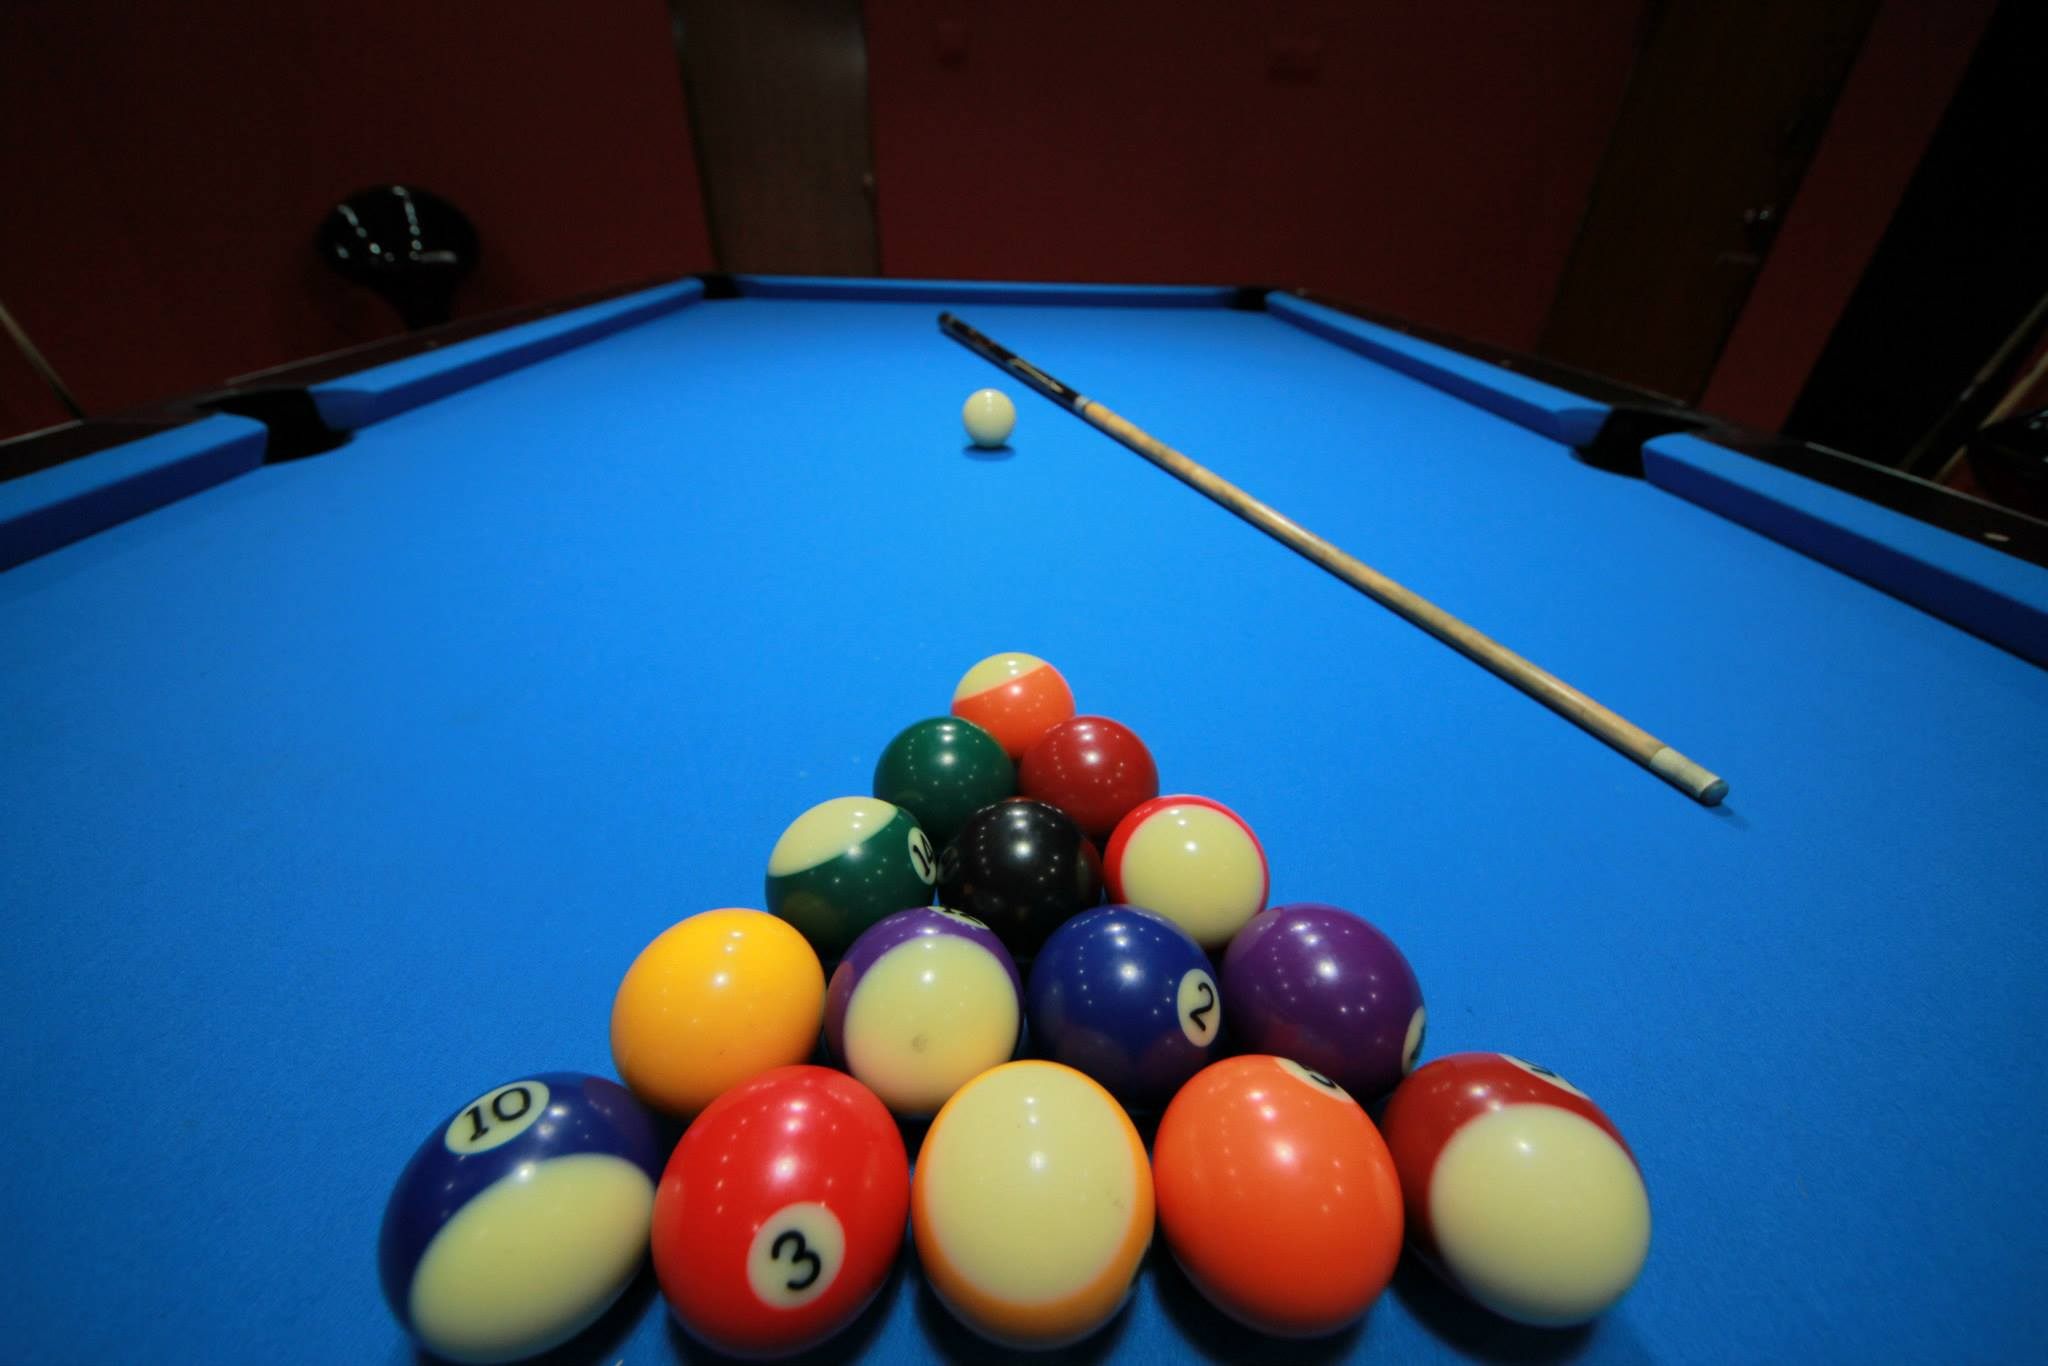
\includegraphics[scale=0.1]{Figures/sport.jpg}}
\caption{Pool room}
\label{fig}
\end{figure}

\subsection{Working Environment}
Orbitax has a great working environment in the office space. From color selection to furniture orientation it has been very careful to create an environment that actively enhances the knowledge exchange and collaborative nature of work.The people here are super friendly and co-operative.



\subsection{ Helping the Community}
Orbitax is involved with many efforts in helping the community around us. The world is facing a pandemic , COVID-19. During this pandemic pandemic, Orbitaxians raise funds from their salary to help the people.
\begin{figure}[htbp]
\centerline{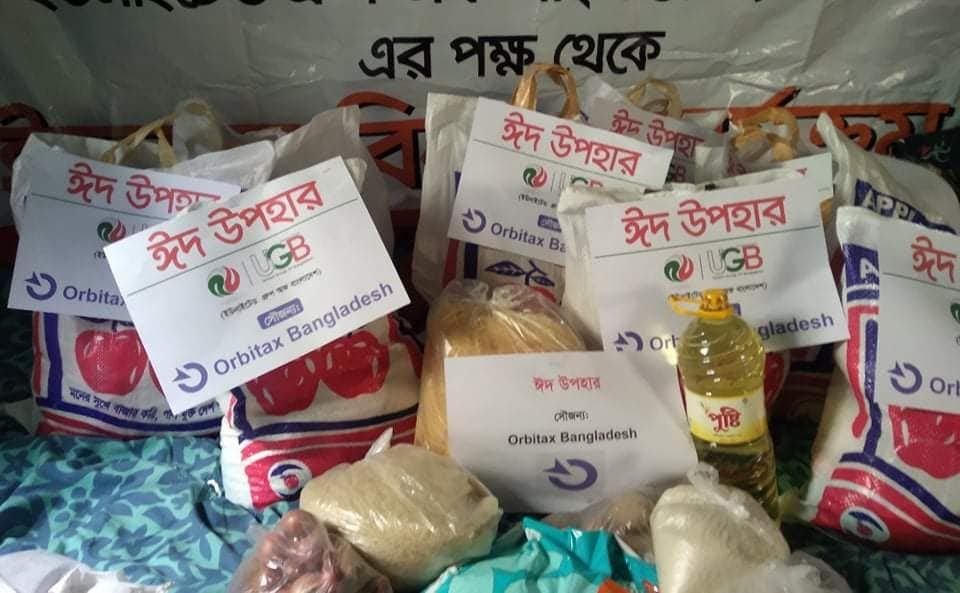
\includegraphics[scale=.5]{Figures/98344888_10157510430898510_3075632179519160320_n.jpg}}
\caption{A small help for the poor people on Eid}
\label{fig}
\end{figure}
 


\subsection{Joining Party}
When a new group of freshers is recruited at Orbitax, A joining party is being held by Orbitax. Here all Orbitaxians celebrate by cutting a cake and welcome the newcomer. I was lucky to have this kind of warm welcome.


\section{The Mega Event}
Every year, Orbitax arranges a tour for the employees. It’s one of the best facilities Orbitax provides to its employees.

\begin{figure}[htbp]
\centerline{
\includegraphics[scale=0.5]{Figures/m.jpg}}
\caption{International tour(Indonesia)}
\label{fig}
\end{figure}

\end{flushleft}

\chapter{Project I involved}
\begin{flushleft}
\label{ch:method}

We were a team of 11 members, 8 interns who are my classmates. And Masud bhai(CTO, Orbitax), Shaon bhai(Senior Software Engineer, Orbitax) And Plabon bhai(Associate Software Engineer, Orbitax) guided us thrugh our six months journey. It was a great experience working with them.


\section{Orbitax Connect}

Orbitax Connect is a mobile application developed for both Android and IOS. It gives a short glimpse of the total Orbitax platform to its user.
 As this project’s information was under NDA so we will talk about its basic overview.
  \begin{figure}[htbp]
\centerline{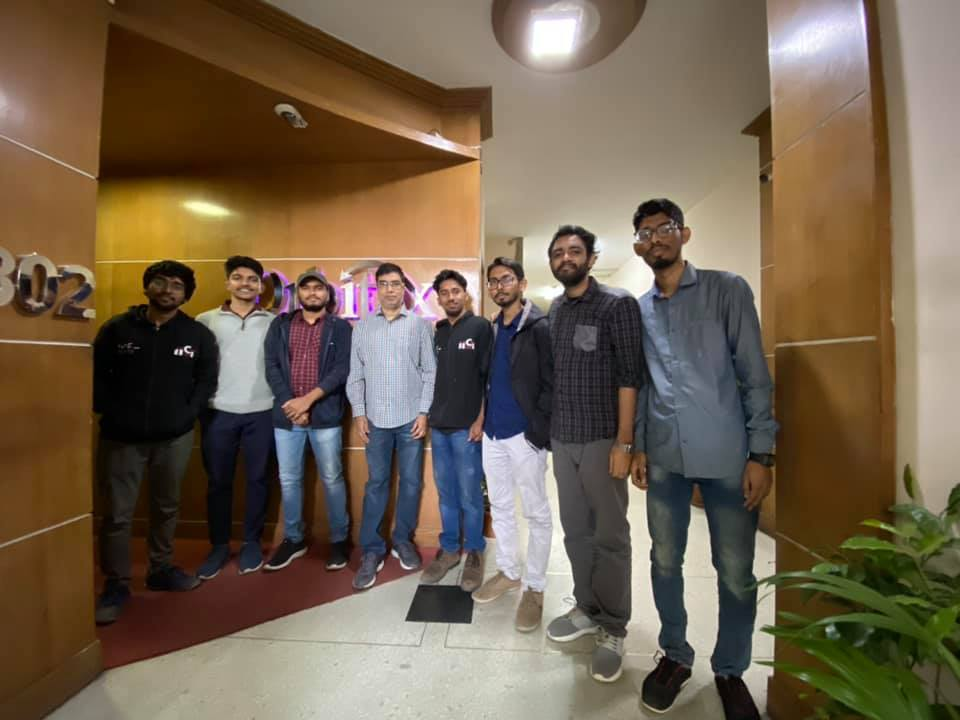
\includegraphics[scale=0.5]{Figures/interns.jpg}}
\caption{Intern team CTO,Orbitax}
\label{fig}
\end{figure}


\subsection{Overview}
Orbitax Connect is a pet project so its development process goes under the tag of a pet project. Being a pet project, orbitax does not compromise its quality, all of the development processes are strictly followed. When I was assigned to this project it’s just in its birth phase. 


\subsection{Team}
We all were assigned to the same project. But we were assigned as a pair. I was assigned with my batchmate Partha Pratim Paul for this project. We work on this project following the pair programming methodology. He was very helpful, hardworking and I got to learn so much from him. It was a pleasant experiance working with him. For some time I was also paired with Ahsan Aziz Ishan who is brilliant and dedicated about his responsibility and I enjoyed working with both of them.


\subsection{Technology}
What technology we used to complete this project are given below:

\begin{enumerate}
    \item Typescript
    \item NodeJs
    \item React
    \item React Native
    \item Redux
    \item Realm
    \item RxJs
    \item Lodash
    \item Jest
    \item Enzyme
    \item Git
    \item Various third party packages
 
\end{enumerate}


\subsection{Features I Was Worked}
I worked on  a library feature where recent tax news and changes reflect on a library system and a home screen where different types of feeds showed with Partha.\\ 

And I also worked in a contact feature where a client can chat,create group and do various things and in this feature I teamed up with Ishan. These were very important features of this project. For implementing these features, I have to learn graphql and implement my learning. I was successfully able to do my work. Besides graphql I used most of the technology mentioned above.


\subsection{Challenges}
The main challenge for me was that I just joined Orbitax and had little idea about industry projects. And I worked with most three people in varsity projects. So working with a big team was a bit challenging at first.  And I don’t have any knowledge of the Orbitax ecosystem. So at first, I have to struggle a little bit to make myself comfortable. After getting used to the ecosystem it’s being pretty comfortable.
The ecosystem of Orbitax is huge so you always find something to learn. The ecosystem is running the microservice architecture. And you will always find a service that does a certain task and it communicates with each other through message passing. As this was my first time with microservice work, so it takes a little bit of time to grasp it. It was a real challenge for me.
Then another thing was maintaining the coding structure. It seems difficult at first. But throughout the time I was comfortable with this. This was fun and the code was much easier to read and understand.
\end{flushleft}
\chapter{Professional Growth}
\begin{flushleft}


\label{ch:results}

Presenting found literature in a useful way

\section{Technology and Tools I Learned}
As Orbitax develops its tools in various technologies. As an intern, I saw them very closely and I had the privilege to learn some of technologies. 


\subsection{Tools}
Programming tools make development easier. In my Intern at Orbitax I have to use the following tools in my daily works:

\begin{itemize}
    \item Webstorm
    \item Visual studio code
    \item React native debugger
    \item Android studio
    \item Xcode
    \item Android and IOS Emulator
    \item Postman
    \item Sublime merge
\end{itemize}

\subsection{Technology}
\subsubsection{RxJs}
RxJS is a library for composing asynchronous and event-based programs by using observable sequences. Think of RxJS as Lodash for events. It’s Reactive Extensions for JavaScript.

 \begin{figure}[htbp]
\centerline{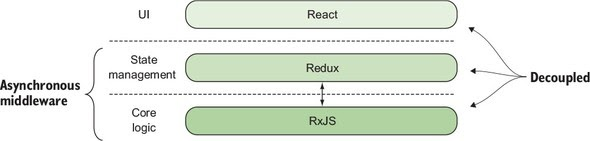
\includegraphics[scale=0.5]{Figures/react.jpg}}
\caption{Layered diagram of the 3R architecture that shows the hierarchy of the different layers of the system}
\label{fig}
\end{figure}

\subsubsection{Redux}
While Redux can be used with any UI layer, it was originally designed and intended for use with React. There are UI binding layers for many other frameworks, but React-Redux is maintained directly by the Redux team.

As the official Redux binding for React, React-Redux is kept up-to-date with any API changes from either library, to ensure that your React components behave as expected. Its intended usage adopts the design principles of React - writing declarative components.

\subsubsection{React Native}
This is a framework for native applications. React Native runs on React, a popular open-source library for building user interfaces with JavaScript. To make the most of React Native, it helps to understand React itself. This section can get you started or can serve as a refresher course.

 \begin{figure}[htbp]
\centerline{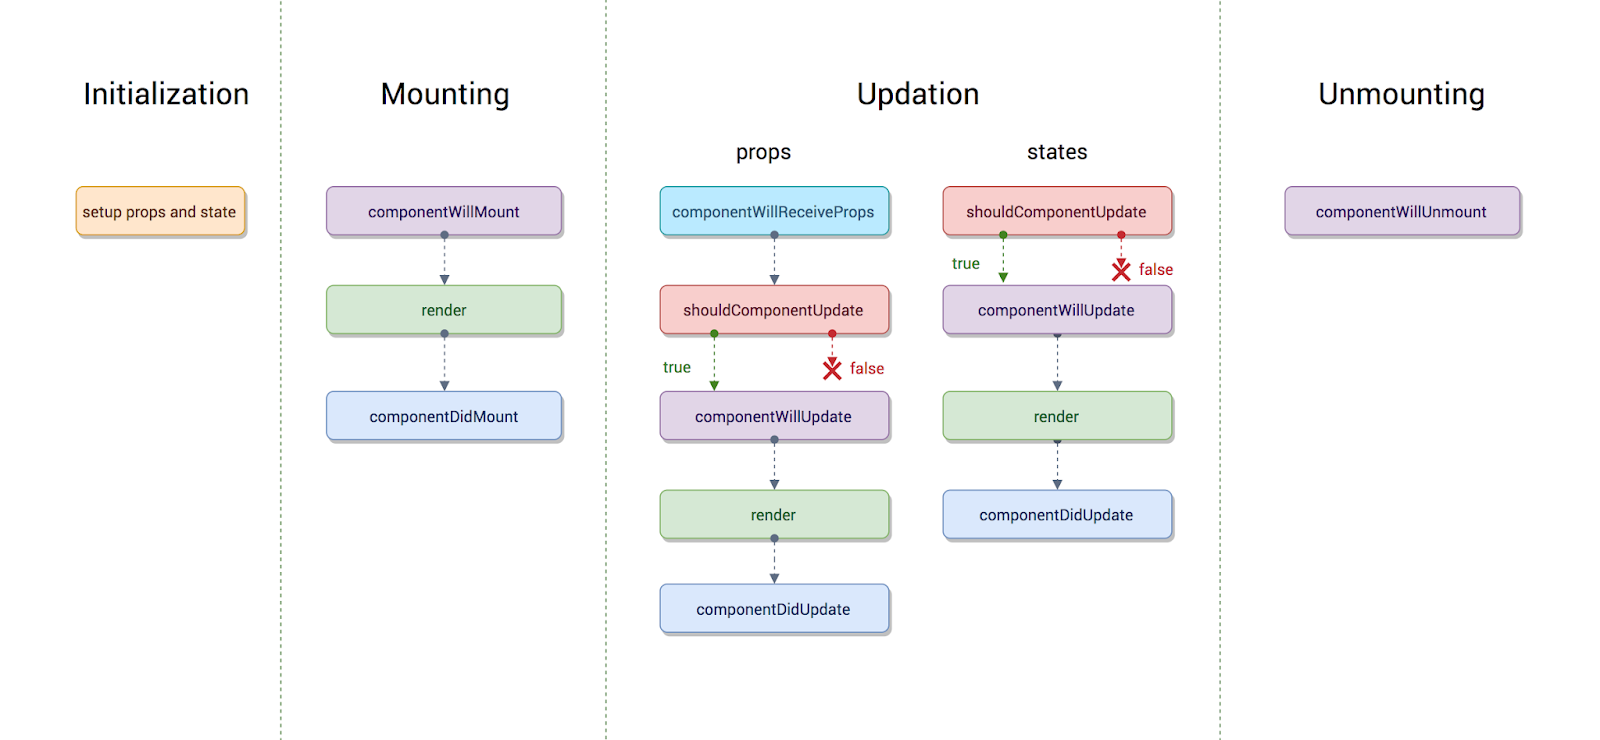
\includegraphics[scale=0.3]{Figures/component.png}}
\caption{React native Component Lifecycle}
\label{fig}
\end{figure}


\section{Development Technique, Pair Programming}
In the Internship, I had the privilege to understand pair-programming perfectly. As I was new to the Orbitax ecosystem, I always had a lot of questions. Therefore, I could clear my confusion while talking with the seniors and gain knowledge about the platform.
Actually, in varsity, we always worked as a team. But never did actual teamwork. In Orbitax, I learned about actual teamwork. Where some developer works in a different part of the same applications.
While working as a pair, we used to work in a way, when my partner was typing I was assisting him, giving him ideas and checking for mistakes; when I was typing my partner was giving me instructions.
Here in Orbitax, I learned that this is an agile programming technique known as Pair Programming. \\
\textit{“Pair programming is an agile software development technique in which two programmers work together at one workstation. One, the driver, types in code while the other, the observer (or navigator), reviews each line of code as it is typed in. The two programmers switch roles frequently.”} \\ 
In Orbitax pair programming is done most of the time and it works as a real technique. Although pair programming is not suitable in all situations, I believe some situations are the most perfect situation for paired programming which are recognized by my experienced team members.

 \begin{figure}[htbp]
\centerline{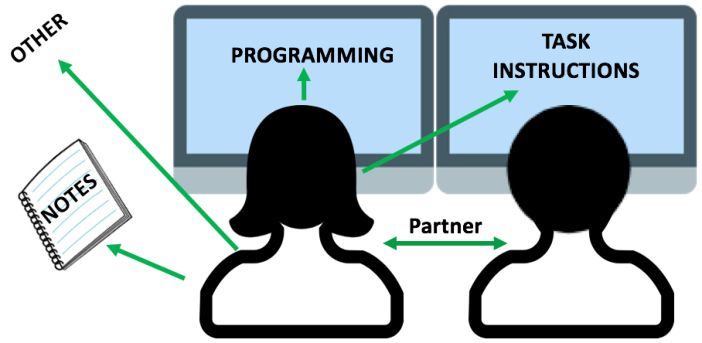
\includegraphics[scale=0.3]{Figures/p.png}}
\caption{Pair Programming}
\label{fig}
\end{figure}

\subsection{Benefits and Costs of pair programming}
Some studies suggest that pair programming produces software with fewer bugs than software developed alone. Reduction in defect rates of 15 percent to 50 percent, varying depending on programmer experience and task complexity. Pairs typically find more design alternatives than programmers working alone, and arrive at simpler, more-maintainable design; they also catch design defects early. Pairs usually complete work faster than one programmer assigned to the same task. \\ 

However, some other studies suggest that pair programming is not uniformly beneficial or effective because although it produces faster, the total programmer time in pair programming is usually higher than that of programming alone.



\section{Professional Learning}
Although technical learning is important, professional learning is the sole purpose of an internship. Orbitax is an excellent place to learn professionalism.

\subsection{No bullying and blaming}
Software development is always teamwork. And in a team, all members don't have similar skills or knowledge. This is true for Orbitax too. During my time of internship, I have made many mistakes like did not maintain code structure. And sometimes stuck in a problem for many hours. But my team leader had never been harsh with me. He always encouraged me to ask for help when I was stuck for some hour. But he did not solve the problem himself unless it was necessary. He always suggests an approach for how to solve that problem. He always encourages us to dig into the error. \\ 
In Orbitax,  I have never seen team leaders and project managers bully people working under their supervision.  \\ 
This practice is effective to keep the work environment healthy. Blaming others for their mistakes does not solve the problem. It only makes the situation and the relationship between coworkers worse.



\subsection{Always Complete your work}
At Orbitax, Everyone is assigned to a particular work and he does his work in his way. At times of scrum, everyone shares their progress with others. All the projects are done in this way. 

\subsection{ Appreciate success, do not discourage for failure}
 The team I have been assigned to has taught me the value of appreciation. Here, the members appreciate each other on their successful contribution to the company and also on their success in some other fields.  
The employees do not discourage people from failure in a particular task. People who can have expertise in that field help others. \\ 
Orbitax gives time to its employees to learn and work at the same time. It has a really good work environment.

\subsection{Attiude}
Orbitax Ltd. is a Software Company with full of fun and creative and Orbitaxians are very much friendly. As an intern, these attract me very much and I always try to follow them to be a successful Software Engineer as well as a successful man.

\subsection{ Quality of work}
Orbitax Ltd. follows a great standard of pure software engineering and its product quality is very high. Time to time code is reviewed so that better quality software is developed. I tried to maintain the standard of work from my side. \\
They have a really good reputation for completing a very complex time within a short period maintaining the quality and architecture of code.

\subsection{Negotiation}
Negotiation is an important part of software engineering. At Orbitax, I have had practical experience in negotiation. We, the developers here, negotiate with our product owner and domain expert quite often here. I also had such an experience and could create a win-win situation.
\subsection{Planning before doing}
Before starting to implement a product, the assigned developer creates a plan under the direct supervision of the Team Leader.
This planning contains almost every detail for the implementation of the product. 
This generally includes : 

\begin{itemize}
\item Understanding the high-level view of the product
\item Architecture to follow
\item Create low-level details for the product
\item Task breakdown
\item What tools to be used 
\item Implementing the base for the product
\item And many more …

\end{itemize}


\section{Organizing}
One of the best ways of learning how to organize is to start organizing oneself of his/her own and after spending almost six months at Orbitax I should say that I am a much more organized person only by practicing that principle. And now being organized, I can say that I am ready to organize others.
\end{flushleft}
\chapter{Conclusion}
\begin{flushleft}
\label{ch:discussion}

\section{Conclusion}
The six months of Internship was a time of experimentation. Internship in an intermediate period of the academic calendar is exceptional from the perspective of our country. From that point of view, this is a matter of glory that during the internship I have passed the best academic period in my life by experiencing real-world technology. It is a matter of grandeur that what I read yesterday at the book is now available to me. Moreover, gathering a vast knowledge about how the real-world works can help me to prepare myself for an upcoming working life for me.
I would like to convey my thanks to the Institute of Information and Communication Technology, Shahjalal University of Science, and Technology for providing me an opportunity to gain an idea of the competitive environment in the professional field. It has certainly lifted my software development skills in terms of design and coding. I now look forward to facing the upcoming challenges of the world.
Orbitax Ltd. is a leading software company in Bangladesh with its innovative and reputed products. So, it was a great opportunity for me to complete my internship period as an effective member of the development of Orbitax. Concerning the assigned project work I had, it was interesting to implement something else that I was taught in my bachelor program. It was interesting to me from different points of view. It was a real pleasure to work in an office with corporate culture. Moreover, working in a team and a friendly official environment made me learn different things. Even though that was something new for me, I was able to change myself with this. Different tools and technologies, experienced human resources, a large range of business domains, innovative products, inspirational and motivating higher authority and friendly environment were the most significant factors to learn professionalism, positive attitude, winning mentality, self- initiative, team strength.

In a word, this internship was a great experience for me. And I hope that this experience will give me inspiration and instruction to build up to me a better future.

\end{flushleft}

\begin{thebibliography}{9}
\bibitem{orbitax} 
"Orbitax":: About us \href{https://www.orbitax.com/about/}{https://www.orbitax.com/about}

\bibitem{reactnative} 
"Reac Native" \href{https://reactnative.dev/}{https://reactnative.dev}

\bibitem{dotnet} 
"Asp DotNet core" \href{https://dotnet.microsoft.com/}{https://dotnet.microsoft.com/}

\bibitem{redux} 
"Redux" \href{https://redux.js.org/introduction/getting-started}{https://redux.js.org/introduction/getting-started}

\bibitem{type} 
"TypeScript" \href{https://www.typescriptlang.org/}{https://www.typescriptlang.org/}

\bibitem{rxjs} 
"RxJs" \href{http://reactivex.io/}{http://reactivex.io/}

\end{thebibliography}



\pagestyle{plain} 

%Literaturverzeichnis
\newpage
\printbibliography
\addcontentsline{toc}{chapter}{Bibliography}
%\ifuseGermanVersion
%	\bibliographystyle{fhstp-apalike}
%\else
%    \bibliographystyle{apa-good}
%\fi

%\bibliography{Bibliography.bib}

% Bilderverzeichnis
% \newpage
% \listoffigures
% \addcontentsline{toc}{chapter}{List of Figures}
% % Tableverzeichnis
% \newpage
% \listoftables
% \addcontentsline{toc}{chapter}{List of Tables}
% %Codelistingsverzeichnis
% \newpage
% \lstlistoflistings
% \addcontentsline{toc}{chapter}{List of Listings}
% \newpage

% ============================================

% \include{Chapters/Appendix}


% ============================================

\end{document}























